\NewDocumentCommand{\drawunit}{mm}
{
    \lPoint{O}{#1}
    \lShift{A}{O}{#2:-0.12}
    \draw[rotate=#2,-stealth,thin](A) arc (180:540:0.12 and 0.24);
    \lShift{B}{O}{#2:0.3}
    \draw[-latex,gray,ultra thin] (O)--(B);
}

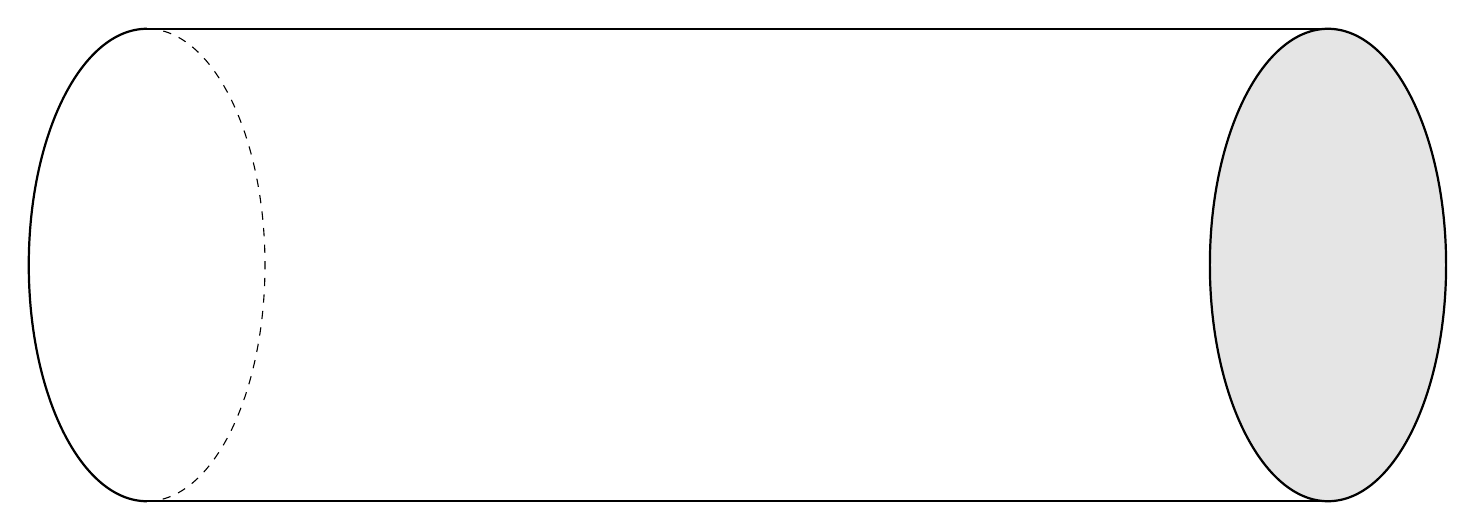
\begin{tikzpicture}[scale=1.5]
    \foreach \i in {-5,-4,...,5}
    {
        \foreach \j in {-1.2,-0.4,0.4,1.2}
        {
            \drawunit{\i,\j}{0}
        }
    }
    \draw[thick](+5,0) ellipse (1 and 2);
    \draw[thick](-5,2) arc (90:270:1 and 2);
    \draw[dashed](-5,2) arc (90:-90:1 and 2);
    \draw[thick] (-5,+2)--(+5,+2);
    \draw[thick] (-5,-2)--(+5,-2);
    \fill[fill=black,fill opacity=0.1](+5,0) ellipse (1 and 2);
\end{tikzpicture}
